% Candidate insertions only. This file is not included by the manuscript.
% Requires graphicx. Paths assume compilation from paper_www2027/.
% Short captions below require the shared setup in SETUP_SNIPPET.tex.
% Full standalone caption alternatives are in CAPTIONS_AND_ACCESSIBILITY.md.

% Candidate for Introduction Figure 1 after author review; keep the existing turquoise-chair figure and manuscript reference unchanged.
\begin{figure}[t]
\centering
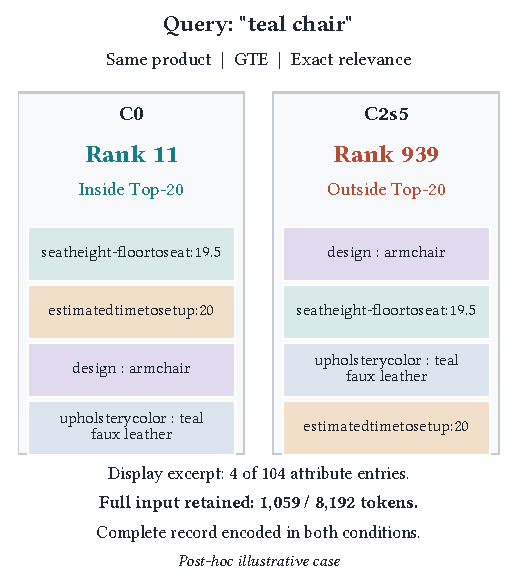
\includegraphics[width=\columnwidth]{../revision_evidence_20260917/figure_revision/figures/figure1_teal_chair_candidate.pdf}
\caption{Example of target-only attribute-order sensitivity: the same fully retained product input ranks 11th or 939th, crossing the Top-20 cutoff.}
\Description{Two independent cards compare the same Exact-labeled WANDS product for query teal chair with GTE. C0 has rank 11, inside Top-20; C2s5 has rank 939, outside Top-20. The cards contain the same four complete attribute entries with matching colors: seat height 19.5, estimated setup time 20, design armchair, and upholstery color teal faux leather. Their order changes. The display is an excerpt of 104 entries; both conditions encode the complete 1,059-token record. The figure is labeled post-hoc illustrative case and contains no deployment timeline or product photograph.}
\label{fig:revision-figure1-teal-chair-candidate}
\end{figure}

% Section 3, adjacent to the intervention and candidate-inclusion state definitions.
\begin{figure*}[t]
\centering
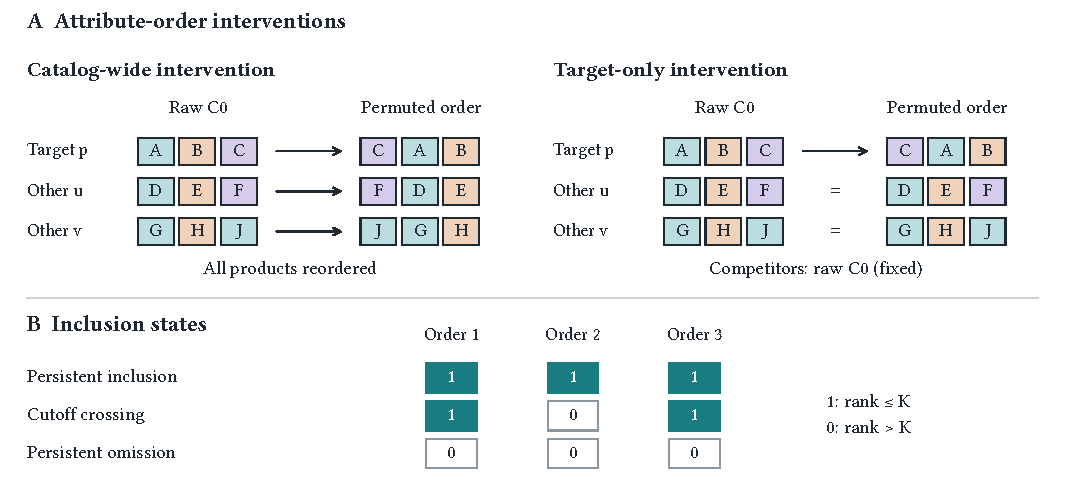
\includegraphics[width=\textwidth]{../revision_evidence_20260917/figure_revision/figures/figure2_intervention_and_states.pdf}
\caption{Attribute-order interventions and candidate-inclusion states over a finite family of orderings.}
\Description{Two intervention diagrams each contain a target and two other products. Colored letter blocks denote complete attribute entries. Every product is reordered in the catalog-wide panel; only the target is reordered in the Target-only intervention panel, and both competitors stay at raw C0. Below, binary rows 111, 101, and 000 show persistent inclusion, cutoff crossing, and persistent omission. One denotes rank at most K. The diagram contains no measured proportions.}
\label{fig:revision-figure2-intervention-and-states}
\end{figure*}

% Results / RQ1, main text.
\begin{figure*}[t]
\centering
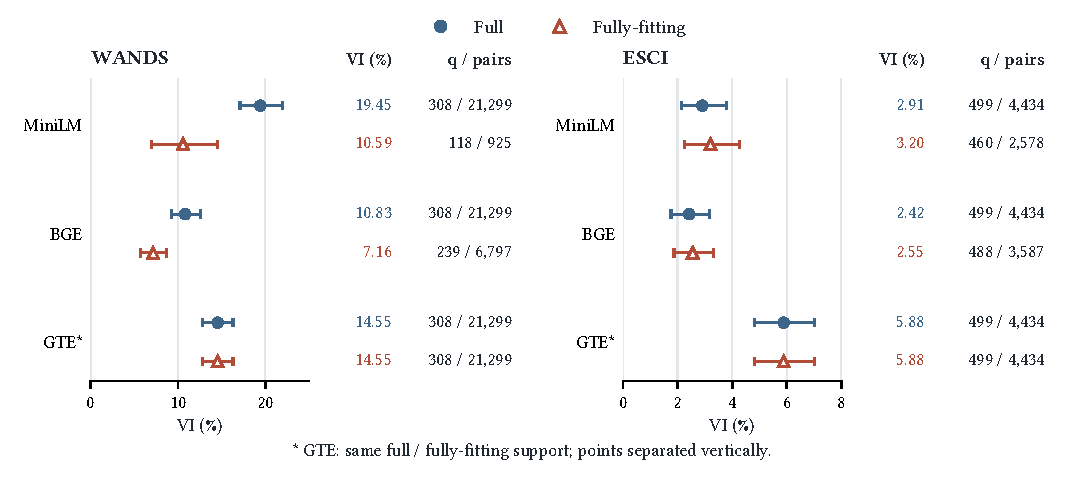
\includegraphics[width=\textwidth]{../revision_evidence_20260917/figure_revision/figures/rq1_vi_top20_main.pdf}
\caption{Target-only inclusion instability for full and fully-fitting target populations, with fixed competitors.}
\Description{Two panels show Top-20 VI with horizontal 95\% intervals for WANDS and ESCI, each with MiniLM, BGE, and GTE. Filled circles denote full targets, open triangles fully-fitting targets. Each estimate has a numeric VI percentage and query/pair count. Full/fitting VI percentages are WANDS MiniLM 19.45/10.59, BGE 10.83/7.16, GTE 14.55/14.55; ESCI MiniLM 2.91/3.20, BGE 2.42/2.55, GTE 5.88/5.88. GTE points are separated vertically despite identical support and intervals. All competitors remain raw C0.}
\label{fig:revision-rq1-vi-top20-main}
\end{figure*}

% Appendix, with a cross-reference from Results / RQ1.
\begin{figure*}[t]
\centering
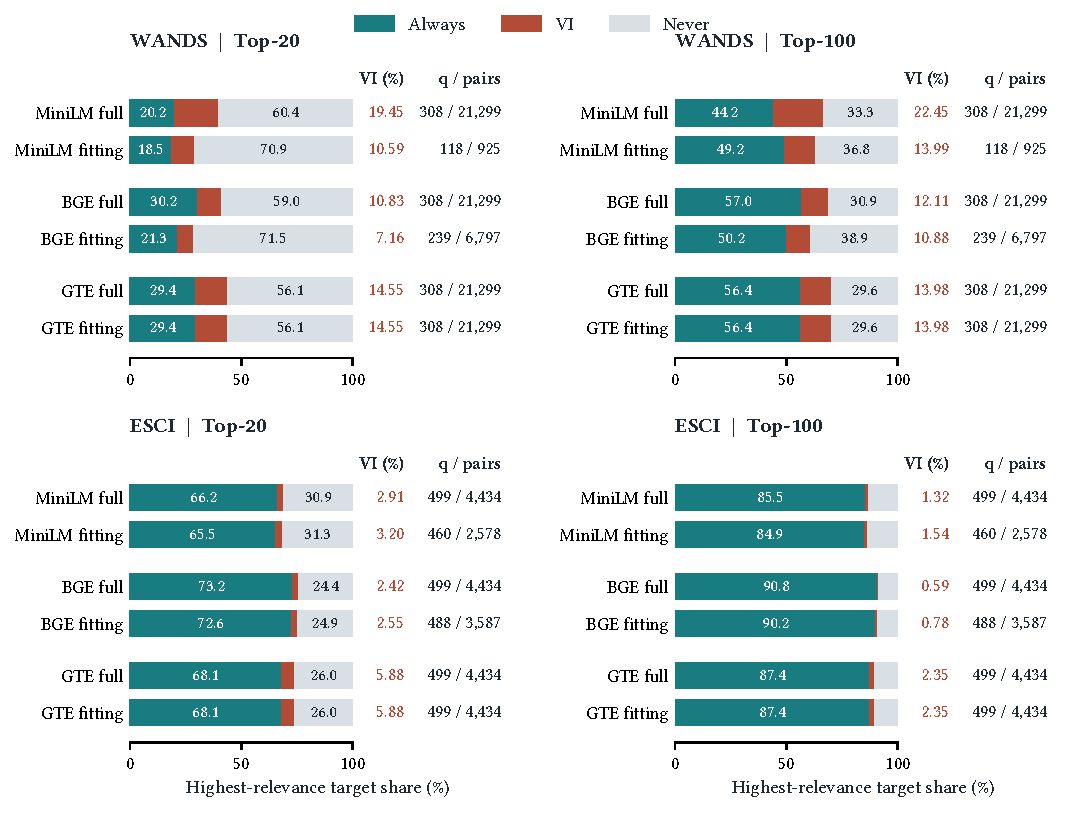
\includegraphics[width=\textwidth]{../revision_evidence_20260917/figure_revision/figures/rq1_states_top20_top100_appendix.pdf}
\caption{Persistent inclusion, cutoff crossing, and persistent omission for full and fully-fitting targets.}
\Description{Four stacked-bar panels compare two target supports for each encoder at Top-20 and Top-100 on WANDS and ESCI. Teal is Always, rust is VI, and gray is Never. A numeric VI column makes every cutoff-crossing proportion visible, including WANDS BGE fully-fitting 7.16 percent at Top-20. Each row also lists eligible queries and highest-relevance pairs. The complete raw C0 competitor catalog stays fixed.}
\label{fig:revision-rq1-states-top20-top100-appendix}
\end{figure*}

% Results / RQ2, main text.
\begin{figure*}[t]
\centering
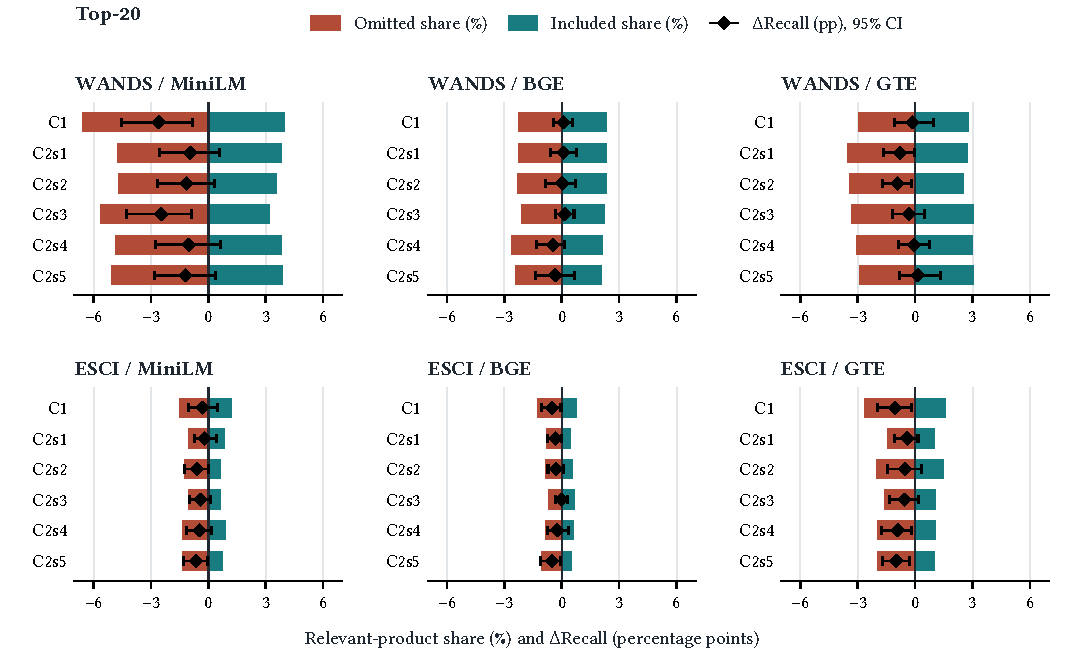
\includegraphics[width=\textwidth]{../revision_evidence_20260917/figure_revision/figures/rq2_membership_top20_main.pdf}
\caption{Relevant-product gains and losses under attribute permutations at Top-20. Diamonds show net Recall changes with 95\% query-bootstrap intervals.}
\Description{Six Top-20 panels cross two datasets with three encoders. Each has six horizontal bar pairs, C1 and C2s1 through C2s5 versus C0. Rust bars extend left for omitted relevant-product shares and teal bars extend right for included shares, in percent. Black diamonds show net Recall changes in percentage points with paired 95\% intervals. Every panel uses the same minus seven to plus seven scale. This is catalog-wide membership evidence; exact within-query cancellation is reported separately in the companion table.}
\label{fig:revision-rq2-membership-top20-main}
\end{figure*}

% Appendix, with a cross-reference from Results / RQ2.
\begin{figure*}[t]
\centering
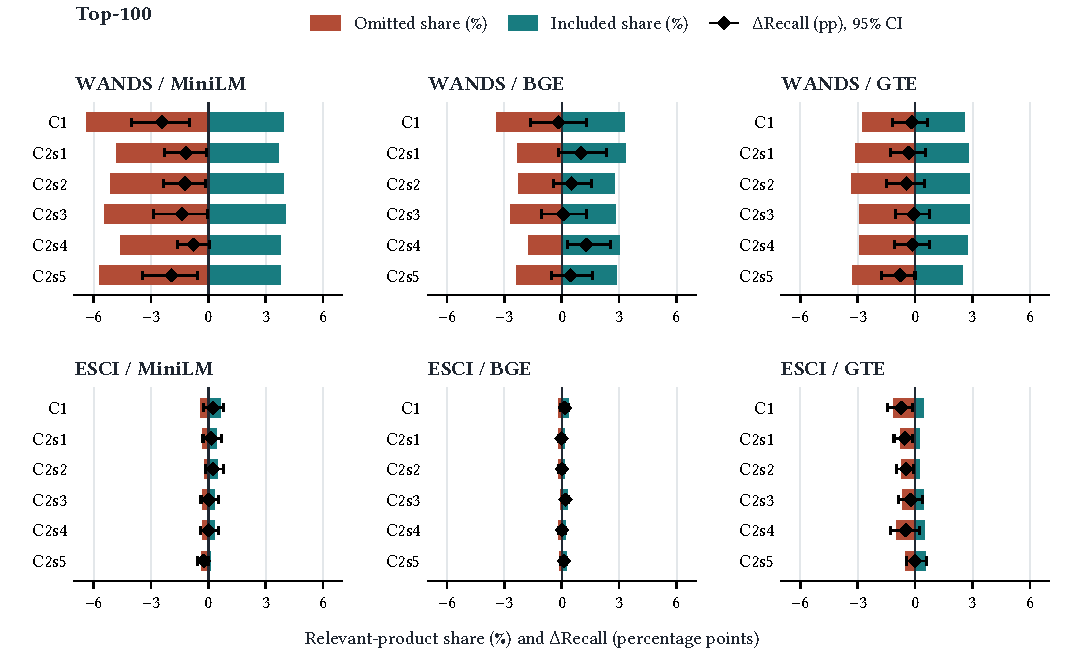
\includegraphics[width=\textwidth]{../revision_evidence_20260917/figure_revision/figures/rq2_membership_top100_appendix.pdf}
\caption{Relevant-product gains and losses under attribute permutations at Top-100. Diamonds show net Recall changes with 95\% query-bootstrap intervals.}
\Description{Six Top-100 panels cross two datasets with three encoders. Each has six horizontal bar pairs, C1 and C2s1 through C2s5 versus C0. Rust bars extend left for omitted relevant-product shares and teal bars extend right for included shares, in percent. Black diamonds show net Recall changes in percentage points with paired 95\% intervals. Every panel uses the same minus seven to plus seven scale. This is catalog-wide membership evidence; exact within-query cancellation is reported separately in the companion table.}
\label{fig:revision-rq2-membership-top100-appendix}
\end{figure*}

% Results / RQ2, beside the Top-20 membership figure. Prefer the supplied native LaTeX table.
\begin{figure}[t]
\centering
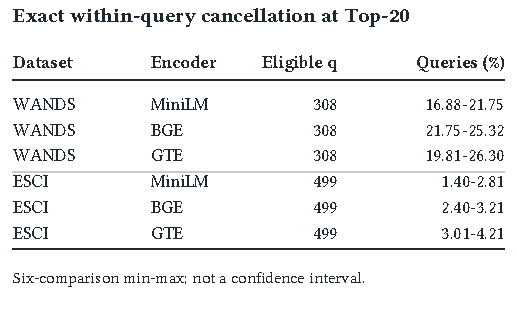
\includegraphics[width=\columnwidth]{../revision_evidence_20260917/figure_revision/figures/rq2_cancellation_top20_table.pdf}
\caption{Exact within-query cancellation across six attribute-order comparisons at Top-20.}
\Description{A six-row table lists dataset, encoder, eligible queries, and the Top-20 proportion of queries with equal positive gains and losses. WANDS ranges are MiniLM 16.88-21.75, BGE 21.75-25.32, and GTE 19.81-26.30 percent, with denominator 308. ESCI ranges are MiniLM 1.40-2.81, BGE 2.40-3.21, and GTE 3.01-4.21 percent, with denominator 499. Ranges span six existing comparisons and are not confidence intervals.}
\label{fig:revision-rq2-cancellation-top20-table}
\end{figure}
